\documentclass[12pt]{article}
\usepackage[a4paper,margin=1in]{geometry}
\usepackage[T1]{fontenc}
\usepackage{times}
\usepackage[scaled=0.92]{helvet}
\usepackage{mtpro2}
\usepackage[sf,bf]{titlesec}
\usepackage[font=small,width=0.7\textwidth]{caption}
\usepackage{fancybox}
\usepackage{fancyhdr}
\usepackage{rotating}
\usepackage{picins,graphicx}
\usepackage{tikz}
\usetikzlibrary{shapes,arrows}
\usepackage[pdftex]{hyperref}
\title{\sffamily\bfseries Crystallography Service Sample Database Administrator's Guide}
\author{J.P.Hagon\\Computer Systems Support\\School of Chemistry}
\date{\today}
\renewcommand{\abstractname}{Introduction}
\renewcommand{\thefootnote}{\fnsymbol{footnote}}
%
\definecolor{skyblue}{rgb}{0.422,0.648,0.801}
%
% Use these directives to change the appearance of example boxes.
%
\tikzstyle{plainbox} = [draw=blue, fill=skyblue!20, thin,
    rectangle, rounded corners, inner sep=5pt, inner ysep=5pt]
\tikzstyle{exmplbox} = [draw=blue, fill=skyblue!20, thin,
    rectangle, rounded corners, inner sep=5pt, inner ysep=15pt]
\tikzstyle{exmpltitle} =[draw=blue,fill=skyblue!50, text=white, thin]
%
% Headers
%
\pagestyle{fancy}
%
% define tikz block styles for flowcharts
%
\tikzstyle{decision} = [diamond, draw, fill=skyblue!20, 
    text width=7em, text badly centered, node distance=4cm, inner sep=0pt]
\tikzstyle{block} = [rectangle, draw, fill=skyblue!20, 
    text width=5em, text centered, rounded corners, minimum height=4em]
\tikzstyle{wideblock} = [rectangle, draw, fill=skyblue!20, 
    text width=10em, text centered, rounded corners, minimum height=4em]
\tikzstyle{line} = [draw, -latex']
\tikzstyle{cloud} = [draw, ellipse,fill=red!20, node distance=3cm,
    minimum height=2em]
%
\begin{document}
\maketitle
\begin{abstract}
This guide is intended for staff who administer the Newcastle University
Crystallography Service Sample Database.
It includes both a general description of the web interface and 
associated administration procedures along with a more technical
description of the software interface and the database itself so that
administrators can recover from situations such as a forgotton
administrator password.
\end{abstract}
\section{General Description of the System}
\subsection{Introduction}
The system consists of a \emph{front-end} which is used by users
and administrators to submit sample requests and upload analysis data. 
This front-end is implemented using the 
\href{http://www.ruby-lang.org/en/}{ruby} programming language and 
version 3 of \href{http://rubyonrails.org}{Ruby on Rails}.
The front-end is hosted on an \emph{Apache} server running on an
\emph{Ubuntu} linux system. Technical details will be described elsewhere.

The \emph{back-end} consists of a set of ruby programming libraries
and a SQL database --- in this case 
\href{http://www.sqlite.org/}{SQLite3}.
More technical aspects of the back-end will be described elsewhere.

\subsection{Users}

The system has a relatively simple user setup with just one basic user
type. However, there are three levels of authority that a user can have:
\begin{description}
\item[Standard]
Most users of the system will have a standard account which allows them
to submit sample requests and view their own sample data.
\item[Group Leader]
These users have the additional privilege of being able to see all
of the sample data for their own group in addition to their own
samples. A group of users may have more than one designated group leader.
\item[Administrator]
An administrator, in addition to standard user privileges, can do many
administration tasks. These include adding/deleting users, changing user
privileges, submitting/updating/deleting samples, editing public web
pages on the server and uploading files to the server.
\end{description}

Users can either self-register or be added by an administrator.
An administrator can also disable a user account without actually
deleting it.
Only the most basic information about a user is stored in the database,
namely first name, last name and email address. the email address serves
as a login id. The user can set his own password. If the user forgets his
password, the system can email him a secure link to the server via which
the password can be reset.

\subsection{Groups}

All users must be associated with a group. Typically this will be a
research group associated with a particular person. When a user self-registers,
he must select an appropriate group. If such a group does not exist, an
administrator must set one up for him. Usually one or more users will be
designated \emph{group leaders} and will have access to information
about all the group's samples.

\subsection{Samples}

The primary purpose of the system is to track and keep a record of
samples submitted to the crystallography service. A typical workflow is
shown in Figure \ref{fig:sample_workflow}.
Emails are sent automatically by the system when a sample status
is updated by an administrator.

\begin{figure}[!]
\small
\begin{center}
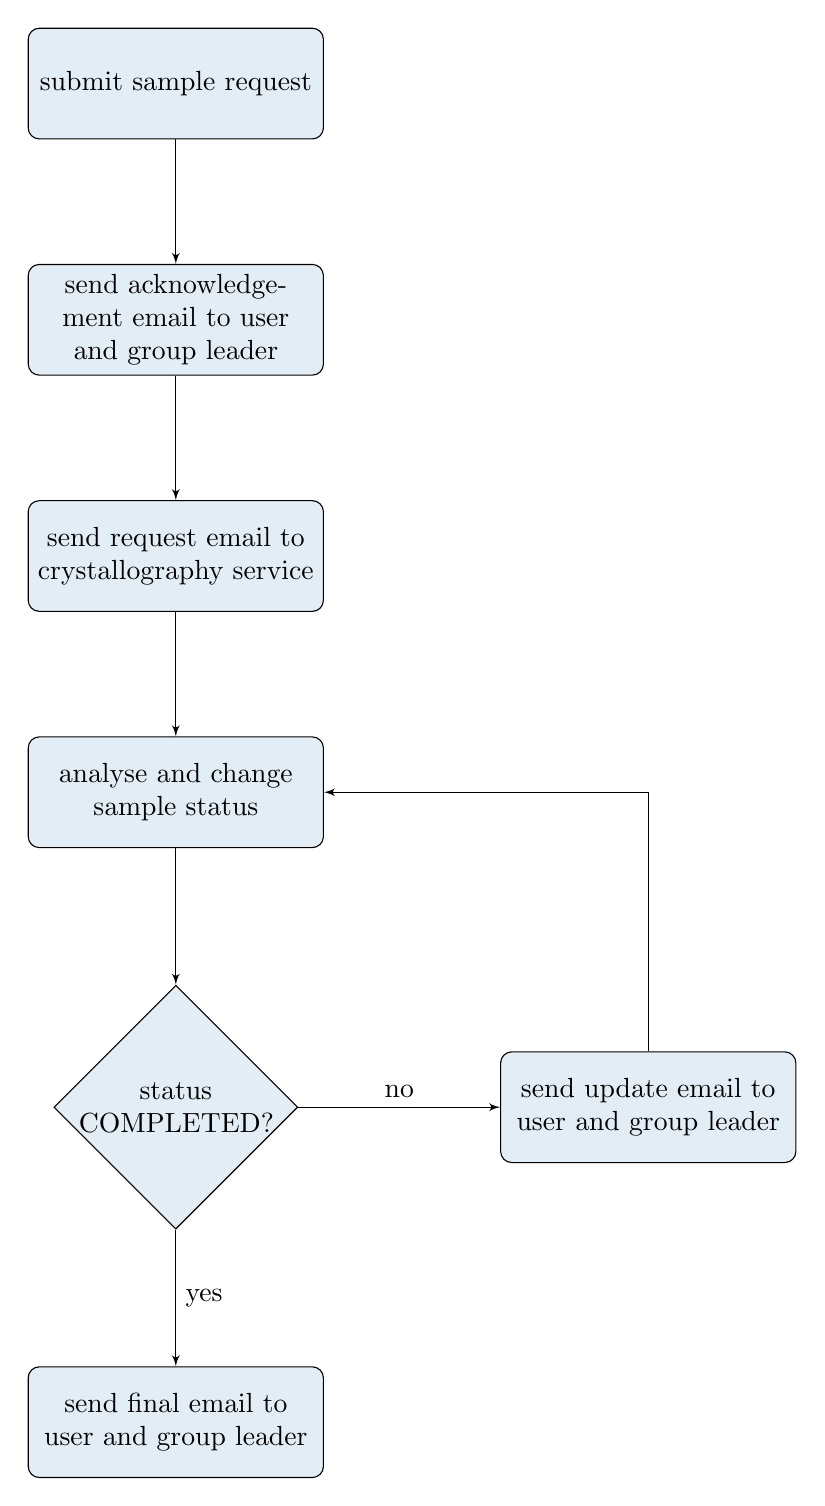
\begin{tikzpicture}[scale=2, node distance = 4cm, auto]
    % Place nodes
    \node [wideblock] (init) {submit sample request};
    \node [wideblock, below of=init, node distance=3cm] (email1) {send acknowledgement email to user
                                          and group leader};
    \node [wideblock, below of=email1, node distance=3cm] (email2) {send request email to
                                          crystallography service};
    \node [wideblock, below of=email2, node distance=3cm] (status) {analyse and change sample status};
    \node [decision, below of=status] (status1) {status\\COMPLETED?};
    \node [wideblock, right of=status1, node distance=6cm] (email4) {send update email to user
                                          and group leader};
    \node [wideblock, below of=status1] (email3) {send final email to user
                                              and group leader};
    % Draw edges
    \path [line] (init) -- (email1);
    \path [line] (email1) -- (email2);
    \path [line] (email2) -- (status);
    \path [line] (status) -- (status1);
    \path [line] (status1) -- node [, color=black] {no} (email4);
    \path [line] (status1) -- node [, color=black] {yes}(email3);
    \path [line] (email4) |- (status);
\end{tikzpicture}
\caption{Typical workflow for sample processing cycle.
Emails are sent automatically by the system whenever the status of a
sample is updated.\label{fig:sample_workflow}}
\end{center}
\normalsize
\end{figure}

\subsection{Public Pages}
Most information on the server can be viewed only by registered users.
However, there are some pages which are more generally accessible.
Such pages include the home page, general information pages and
the sample queue. Public pages can be created and edited by an administrator
using tools provided by the server software. rather than write pure
HTML, an administrator can use a text-based markup language called
\href{http://en.wikipedia.org/wiki/Textile_%28markup_language%29}{Textile}
which can produce sophisticated web pages with all the usual constructs
such as headings, paragraphs, floating elements, tables and images.

\section{The Database}
The core of the system is the database which holds information about 
users, samples etc. In this section we describe the whole database
structure (or \emph{schema} in database parlance).

\begin{sidewaysfigure}
\begin{center}
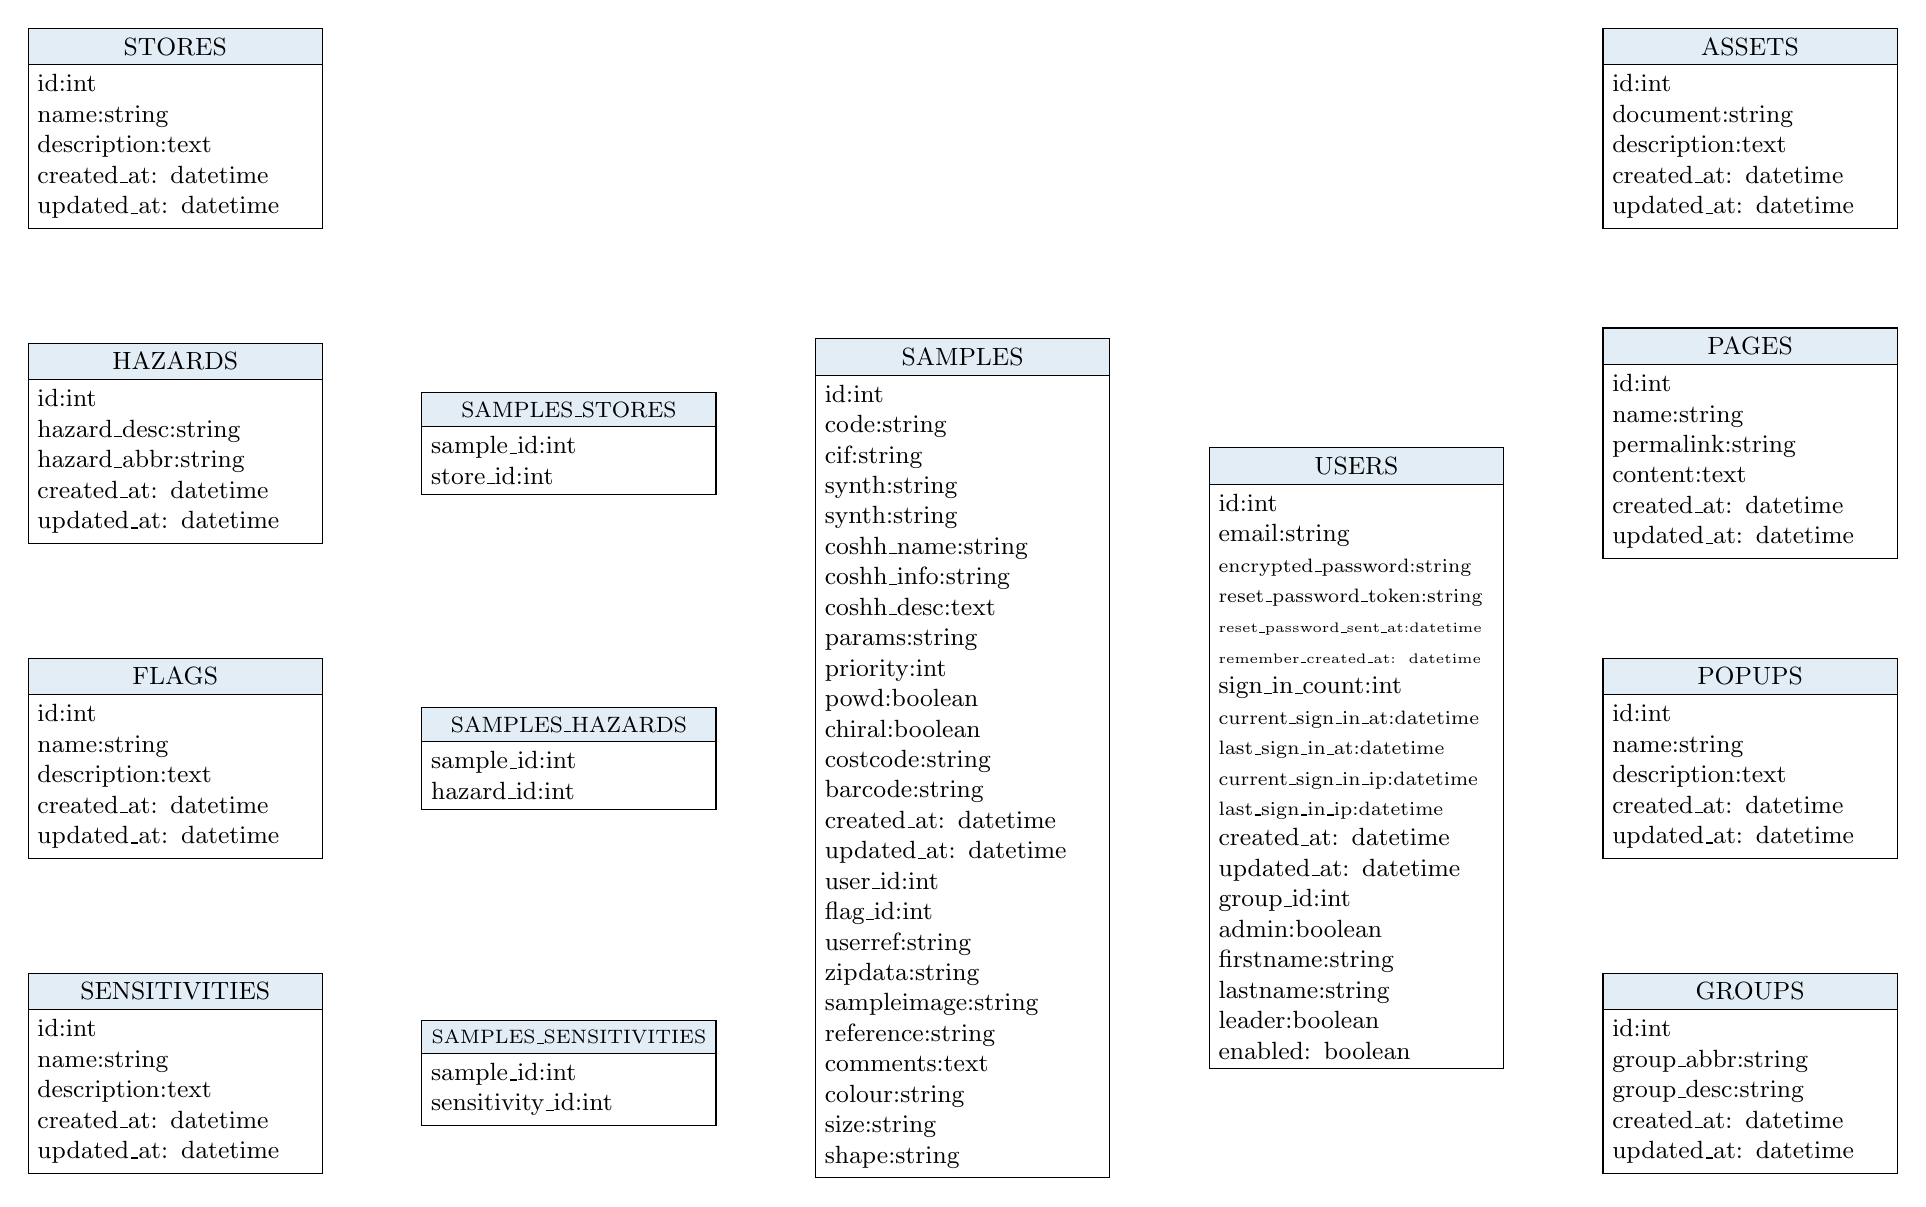
\begin{tikzpicture}[every text node part/.style={text centered}, font=\small]
\tikzset{every node/.style={rectangle split, 
                            rectangle split parts=2, 
                            draw, text width=3.5cm}}
\node(assets) [rectangle split part fill={skyblue!20, white}]
  {ASSETS
  \nodepart{second}
  id:int \\
  document:string \\
  description:text \\
  created\_at: datetime \\
  updated\_at: datetime};

\node(pages) [below of=assets, node distance=4cm, 
              rectangle split part fill={skyblue!20, white}]
  {PAGES
  \nodepart{second}
  id:int \\
  name:string \\
  permalink:string \\
  content:text \\
  created\_at: datetime \\
  updated\_at: datetime};

\node(popups) [below of=pages, node distance=4cm,  
               rectangle split part fill={skyblue!20, white}]
  {POPUPS
  \nodepart{second}
  id:int \\
  name:string \\
  description:text \\
  created\_at: datetime \\
  updated\_at: datetime};

\node(groups) [below of=popups, node distance=4cm,
               rectangle split part fill={skyblue!20, white}]
  {GROUPS
  \nodepart{second}
  id:int \\
  group\_abbr:string \\
  group\_desc:string \\
  created\_at: datetime \\
  updated\_at: datetime};

\node(users) [left of=popups, node distance=5cm,
               rectangle split part fill={skyblue!20, white}]
  {USERS
  \nodepart{second}
  id:int \\
  email:string \\
  {\scriptsize encrypted\_password:string} \\
  {\scriptsize reset\_password\_token:string} \\
  {\tiny reset\_password\_sent\_at:datetime} \\
  {\tiny remember\_created\_at: datetime} \\
  sign\_in\_count:int \\
  {\scriptsize current\_sign\_in\_at:datetime} \\
  {\scriptsize last\_sign\_in\_at:datetime} \\
  {\scriptsize current\_sign\_in\_ip:datetime} \\
  {\scriptsize last\_sign\_in\_ip:datetime} \\
  created\_at: datetime \\
  updated\_at: datetime \\
  group\_id:int \\
  admin:boolean \\
  firstname:string \\
  lastname:string \\
  leader:boolean \\
  enabled: boolean};

\node(samples) [left of=users, node distance=5cm,
               rectangle split part fill={skyblue!20, white}]
  {SAMPLES
  \nodepart{second}
  id:int \\
  code:string \\
  cif:string \\
  synth:string \\
  synth:string \\
  coshh\_name:string \\
  coshh\_info:string \\
  coshh\_desc:text \\
  params:string \\
  priority:int \\
  powd:boolean \\
  chiral:boolean \\
  costcode:string \\
  barcode:string \\
  created\_at: datetime \\
  updated\_at: datetime \\
  user\_id:int \\
  flag\_id:int \\
  userref:string \\
  zipdata:string \\
  sampleimage:string \\
  reference:string \\
  comments:text \\
  colour:string \\
  size:string \\
  shape:string };

\node(samphaz) [left of=samples, node distance=5cm,
               rectangle split part fill={skyblue!20, white}]
  {{\footnotesize SAMPLES\_HAZARDS}
  \nodepart{second}
  sample\_id:int \\
  hazard\_id:int};

\node(sampsen) [below of=samphaz, node distance=4cm,
               rectangle split part fill={skyblue!20, white}]
  {{\scriptsize SAMPLES\_SENSITIVITIES}
  \nodepart{second}
  sample\_id:int \\
  sensitivity\_id:int};

\node(sampsto) [above of=samphaz, node distance=4cm,
               rectangle split part fill={skyblue!20, white}]
  {{\footnotesize SAMPLES\_STORES}
  \nodepart{second}
  sample\_id:int \\
  store\_id:int};


\node(flags) [left of=samphaz, node distance=5cm,
               rectangle split part fill={skyblue!20, white}]
  {FLAGS
  \nodepart{second}
  id:int \\
  name:string \\
  description:text \\
  created\_at: datetime \\
  updated\_at: datetime};

\node(hazards) [above of=flags, node distance=4cm,
               rectangle split part fill={skyblue!20, white}]
  {HAZARDS
  \nodepart{second}
  id:int \\
  hazard\_desc:string \\
  hazard\_abbr:string \\
  created\_at: datetime \\
  updated\_at: datetime};

\node(stores) [above of=hazards, node distance=4cm,
               rectangle split part fill={skyblue!20, white}]
  {STORES
  \nodepart{second}
  id:int \\
  name:string \\
  description:text \\
  created\_at: datetime \\
  updated\_at: datetime};

\node(sensitivities) [below of=flags, node distance=4cm,
               rectangle split part fill={skyblue!20, white}]
  {SENSITIVITIES
  \nodepart{second}
  id:int \\
  name:string \\
  description:text \\
  created\_at: datetime \\
  updated\_at: datetime};

\end{tikzpicture}
\end{center}
\caption{The overall database schema.\label{fig:database_schema}}
\end{sidewaysfigure}
\newpage
\tableofcontents
\newpage
\end{document}
